\section{Використання розроблегоно застосунку}
\label{sec:application-usadge}

Застосунок покликаний допомогти користувачам у пошуку оптимальних маршрутів між потрібними їм пунктами, беручи до уваги різні фактори, такі як відстань, час у дорозі, види транспорту та вподобання щодо розкладу. Завдяки інтуїтивно зрозумілому користувацькому інтерфейсу та потужним алгоритмам пошуку, застосунок має на меті спростити процес планування маршруту та надати користувачам точну та надійну інформацію про маршрут.

Основна мета програми - запропонувати зручний та ефективний спосіб пошуку маршрутів на основі індивідуальних уподобань та вимог. Незалежно від того, чи потрібно вам зорієнтуватися в галасливому місті, дістатися до роботи або спланувати поїздку, додаток оснащений необхідними інструментами, які допоможуть знайти найкращі маршрути, що відповідають потребам користувачів.

Щоб розпочати пошук маршруту, користувачі можуть просто ввести початкову та кінцеву зупинки. Користувачі можуть уточнити пошук, вказавши час відправлення, що дозволяє їм планувати свої подорожі з урахуванням запланованих заходів або очікуваних дорожніх умов.

Результати пошуку представлені в чіткій та інтуїтивно зрозумілій формі, відображаючи рекомендовані маршрути разом з детальною інформацією, такою як орієнтовний час у дорозі, відстань, та будь-яка відповідна інформація про маршрут.

У цьому розділі буде розглянуто різні можливості та функції додатку, надаючи детальні пояснення та покрокові інструкції щодо максимального використання його потенціалу. Наприкінці цього розділу з'явится повне уявлення про те, як використовувати додаток на повну потужність і планувати свої маршрути з легкістю та впевненістю.

%Subsections
\subsection{Огляд користувацького інтерфейсу}
\label{subsec:interface-subsection}

Розуміння інтерфейсу має вирішальне значення, оскільки воно закладає основу для безперешкодної навігації та ефективного використання функцій програми. Цей підрозділ має на меті ознайомится з елементами інтерфейсу, їхнім призначенням і тим, як вони впливають на загальний користувацький досвід.

Завдяки детальному вивченню інтерфейсу користувачі отримають повне уявлення про візуальну ієрархію програми, навігаційні меню, функціональність пошукового рядка, відображення карти та інші інтерактивні елементи. Буде висвітлено інтуїтивно зрозумілі дизайнерські рішення, які були реалізовані для забезпечення простоти використання та швидкого доступу до основних функцій.

У підрозділі аналізу інтерфейсу також обговорюватимуться найкращі практики та поради щодо ефективної навігації та використання елементів інтерфейсу. Користувачі дізнаються, як взаємодіяти з різними компонентами, налаштовувати свої уподобання, а також користуватися комбінаціями клавіш і жестами, щоб покращити загальний досвід роботи.

Заглибившись в аналіз інтерфейсу, можна отримають можливість легко орієнтуватися в додатку і використовувати всі його можливості. Незалежно від того, чи ви новачок, чи досвідчений користувач, цей підрозділ надасть цінну інформацію для оптимізації взаємодії та спрощення процесу планування маршрутів.

Коли користувач вперше заходить на сайт, він бачить початкову сторінку. На ній відображено коротку інформацію про застосунок та кнопку для переходу до пошуку, щоб користувач міг якомога швидше знайти потрібний маршрут.

\begin{figure}[!htp]
	\centering
	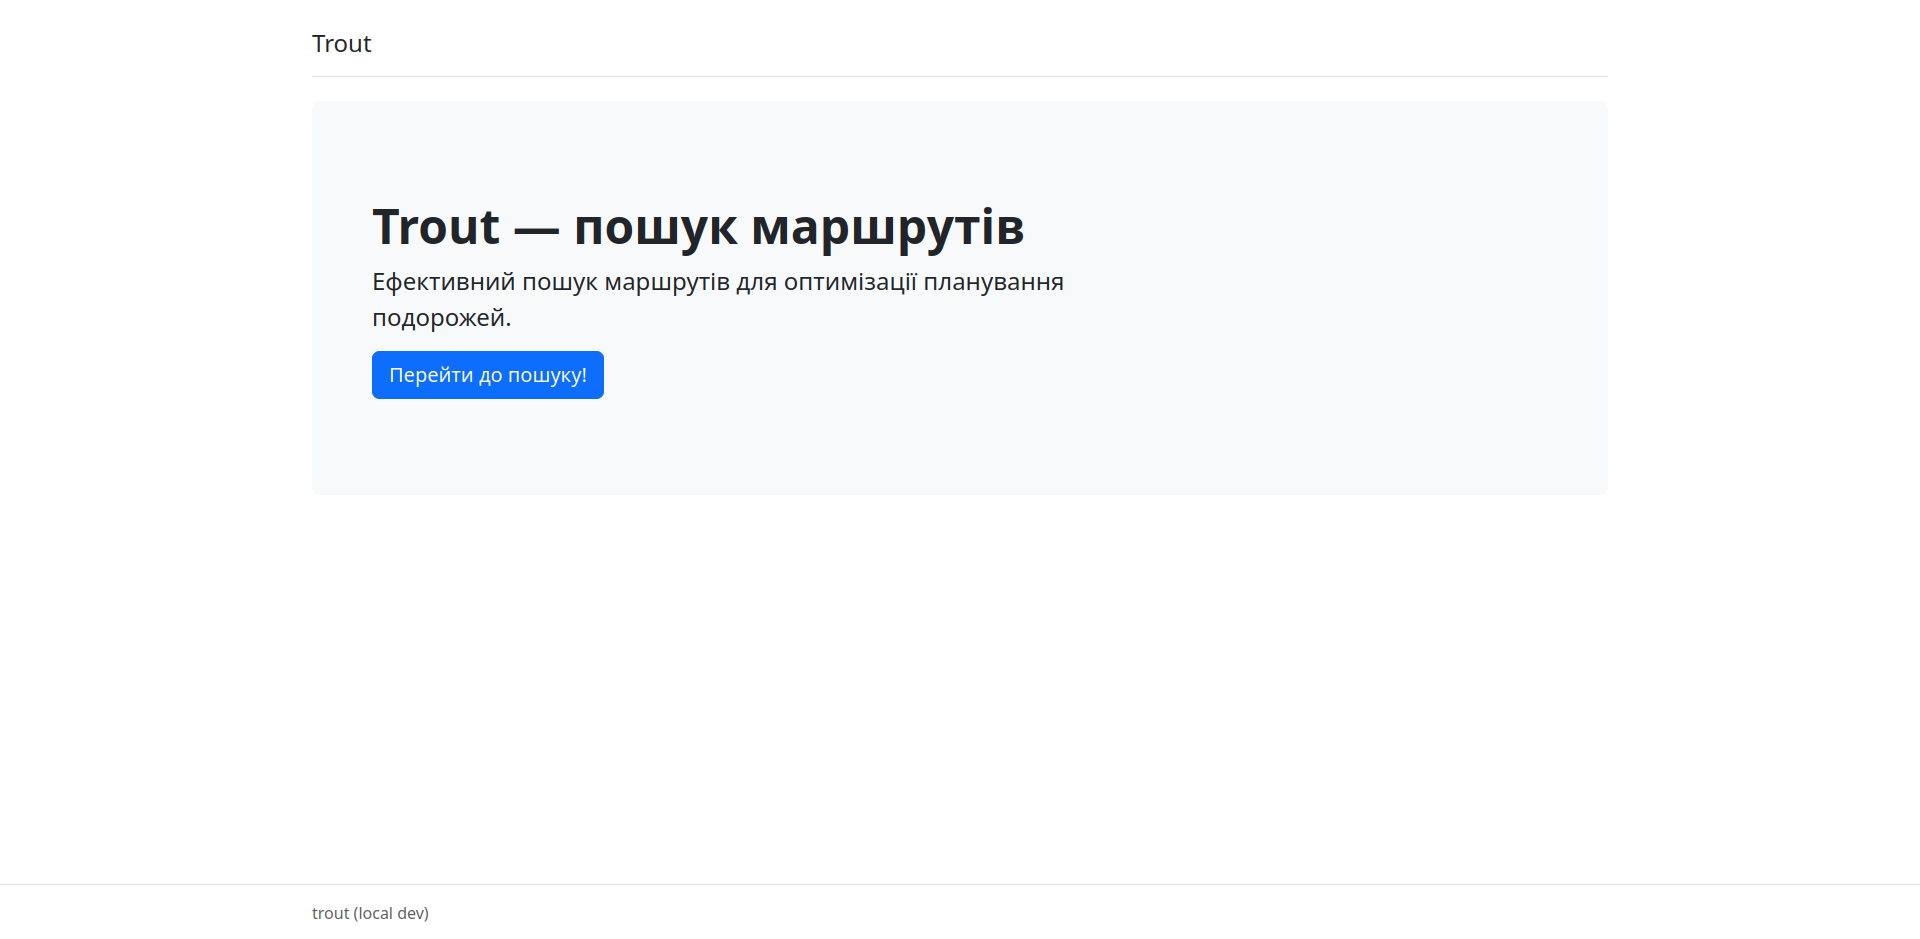
\includegraphics[scale=0.4]{content/chapters/4-results/assets/img/example_mainpage.png}
	\caption{Головна сторінка сайту}
	\label{fig:main_page}
\end{figure}

Завдяки використанню Bootstrap інтерфейс підходить для екранів будь-якого розміру

\begin{figure}[!htp]
	\centering
	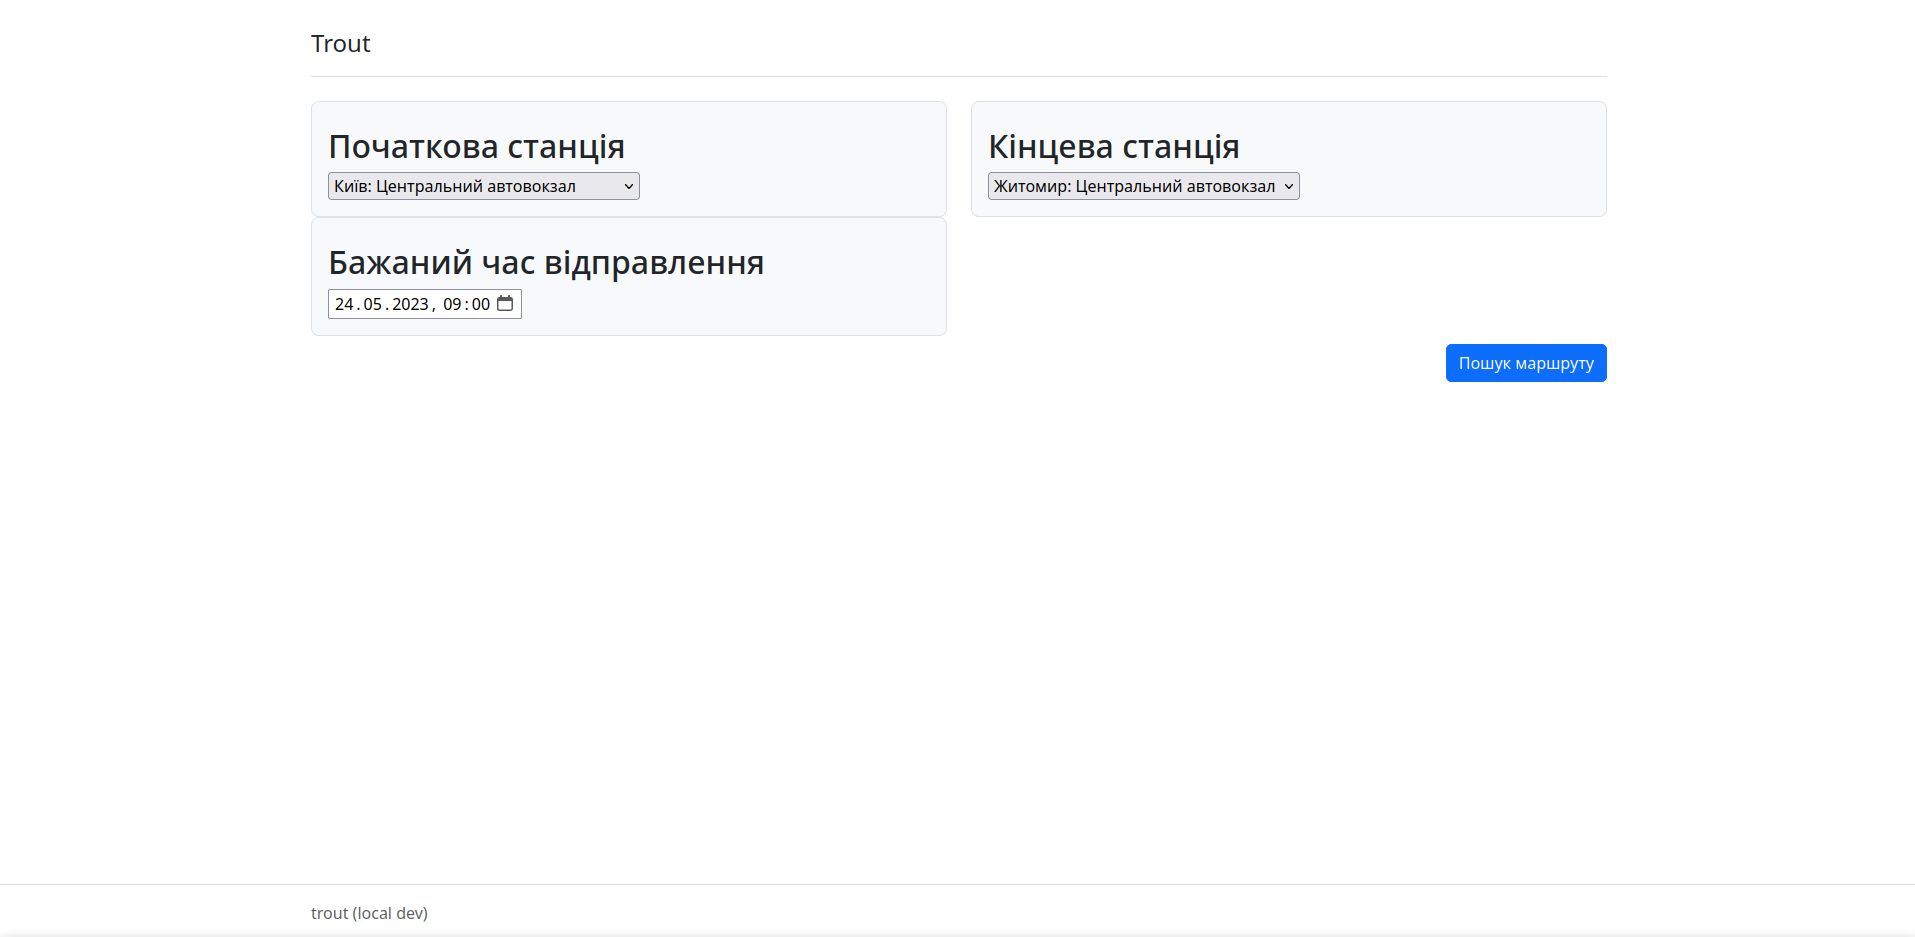
\includegraphics[scale=0.4]{content/chapters/4-results/assets/img/pc_screen.png}
	\caption{Відображення сайту на екрані комп'ютера}
	\label{fig:pc_page}
\end{figure}

\begin{figure}[!htp]
	\centering
	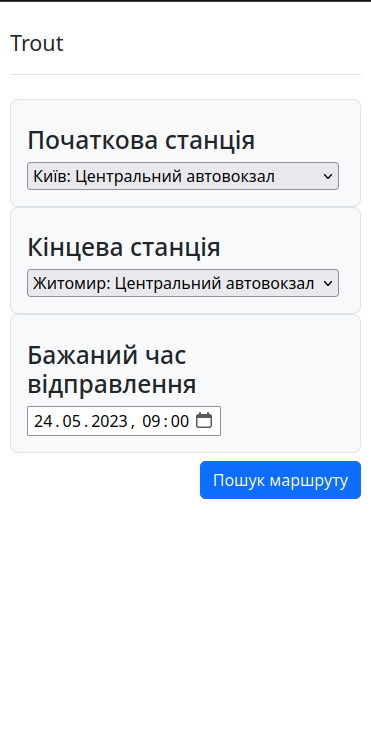
\includegraphics[scale=0.5]{content/chapters/4-results/assets/img/phone_screen.png}
	\caption{Відображення сайту на екрані телефону}
	\label{fig:phone_page}
\end{figure}


\subsection{Огляд функції пошуку маршрутів}
\label{subsec:route-management-subsection}

За допомогою функції пошуку маршруту користувачі можуть ввести початкову та кінцеву зупинки, щоб розпочати процес пошуку. Додаток використовує передові алгоритми для розрахунку найефективніших і найшвидших маршрутів на основі різних факторів, таких як відстань, час у дорозі та час очікування.

Результат пошуку відображається в чіткій та організованій. Маршрут супроводжується детальною інформацією, включаючи приблизний час у дорозі, відстань та покрокові вказівки.

Надаючи комплексну та зручну функцію пошуку маршрутів, застосунок має на меті спростити процес пошуку та навігації оптимальних маршрутів. Незалежно від того, чи користувачі їдуть на роботу, чи досліджують нове місто, чи планують подорож, вони можуть покластися на функцію пошуку маршрутів, яка надасть їм точні, ефективні та надійні варіанти маршрутів.

Пошук маршруту для користувача починається зі сторінки для вводу даних пошуку. На ній користувач може ввести початкову зупинку та кінцеву зупинку, а також бажаний час відправлення.

\begin{figure}[!htp]
	\centering
	
\includegraphics[scale=0.3]{content/chapters/4-results/assets/img/example1_search.png}
	\caption{Сторінка пошуку маршруту}
	\label{fig:search_page}
\end{figure}


Після вводу даних для пошуку, користувач натискає кнопку ``Знайти маршрут''. Застосунок оброблює введені дані, знаходить маршрут та відображає його.

\begin{figure}[!htp]
	\centering
	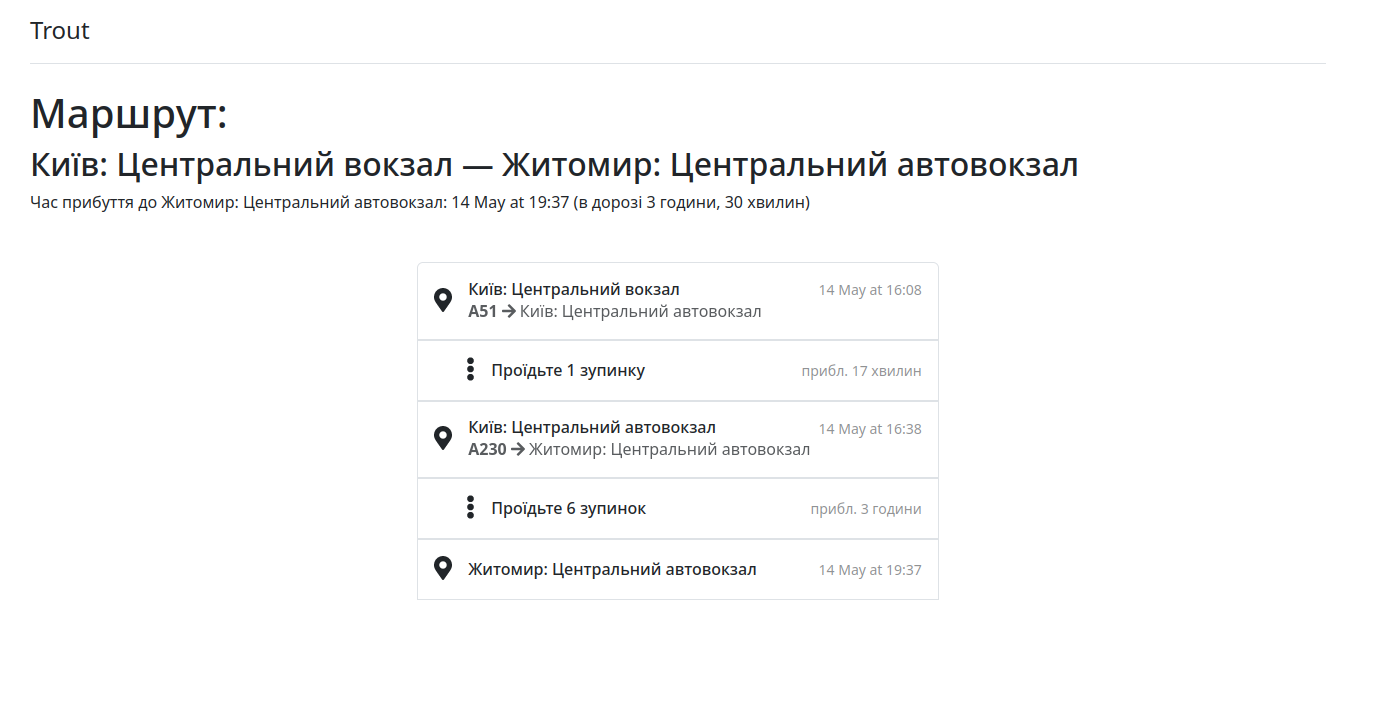
\includegraphics[scale=0.3]{content/chapters/4-results/assets/img/example1_result.png}
	\caption{Сторінка зі знайденим маршрутом}
	\label{fig:route_page}
\end{figure}


Користувач також може переглядати деталі про маршут та зупинки, які входять в знайдений маршрут.

\begin{figure}[!htp]
	\centering
	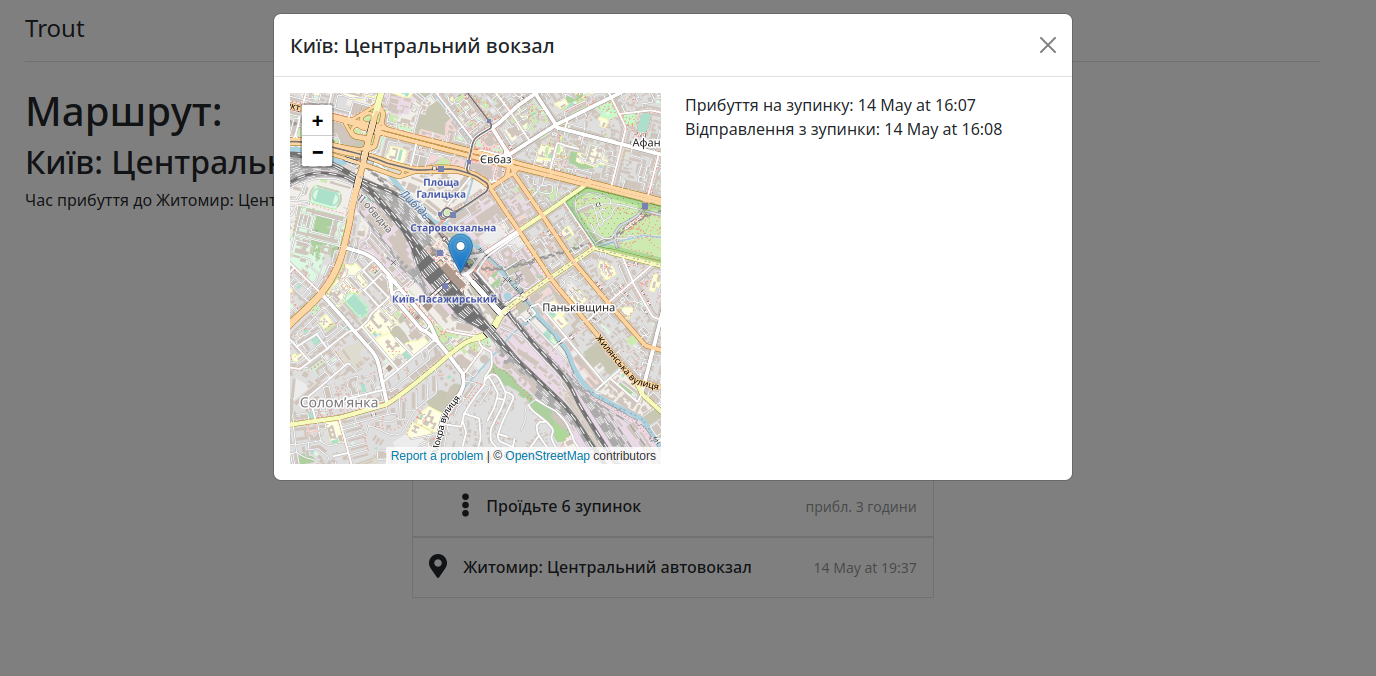
\includegraphics[scale=0.3]{content/chapters/4-results/assets/img/example_station.png}
	\caption{Перегляд деталей про зупинку}
	\label{fig:stop_details_page}
\end{figure}

\begin{figure}[!htp]
	\centering
	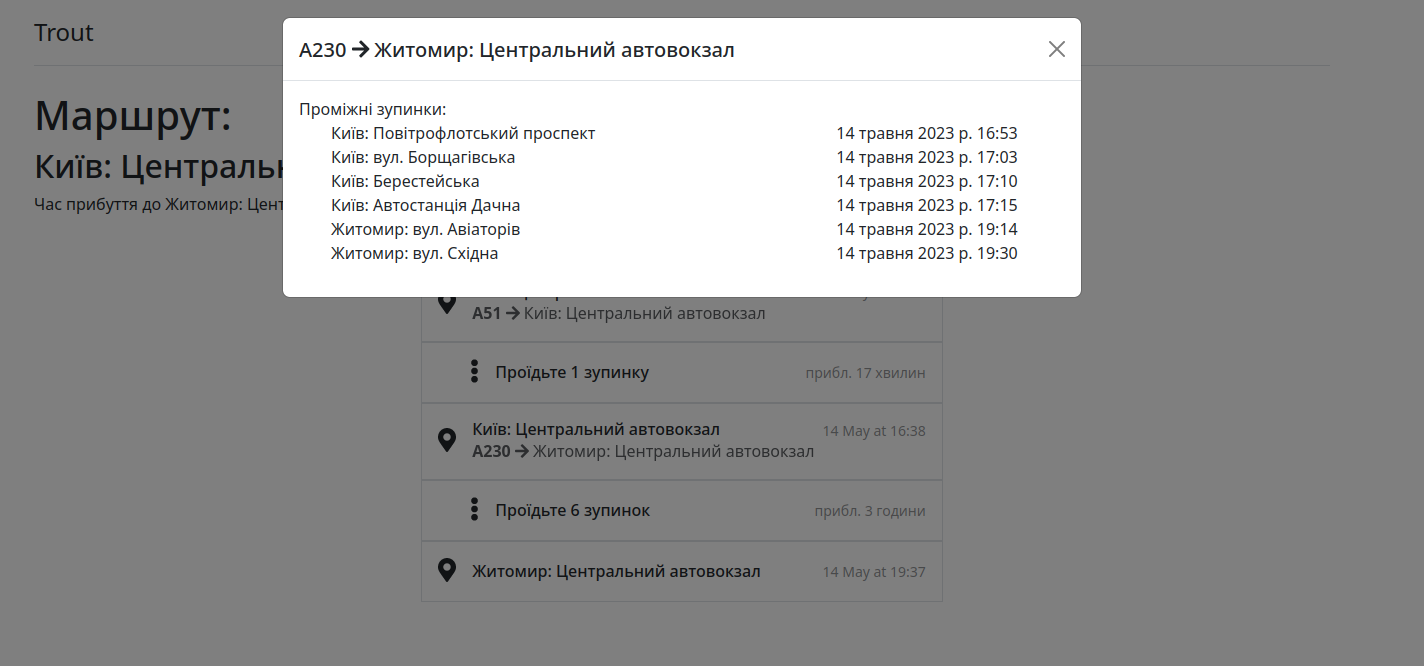
\includegraphics[scale=0.3]{content/chapters/4-results/assets/img/example_stops.png}
	\caption{Перегляд деталей про маршрут}
	\label{fig:route_details_page}
\end{figure}


\subsection{Контроль доступу до управління даними про транспорт}
\label{subsec:route-search-subsection}

Застосунок надає надійну систему облікових записів користувачів, що дозволяє адміністраторам мати спеціальні облікові записи з підвищеними привілеями. Ці облікові записи слугують шлюзами для доступу до адміністративних функцій і можливостей, які недоступні звичайним користувачам. Завдяки окремим обліковим записам адміністраторів програма підтримує чітке розмежування між адміністративними завданнями і взаємодією з користувачами, забезпечуючи ефективне і контрольоване управління системою.

За допомогою облікових записів адміністраторів уповноважений персонал мають можливість створювати, редагувати та видаляти дані про транспортні маршрути.

Функція управління доступом з обліковими записами для адміністраторів дає змогу уповноваженому персоналу ефективно керувати та адмініструвати маршрути транспорту, забезпечуючи безперебійну, безпечну роботу системи відповідно до вимог організації.

\begin{figure}[!h]
	\centering
	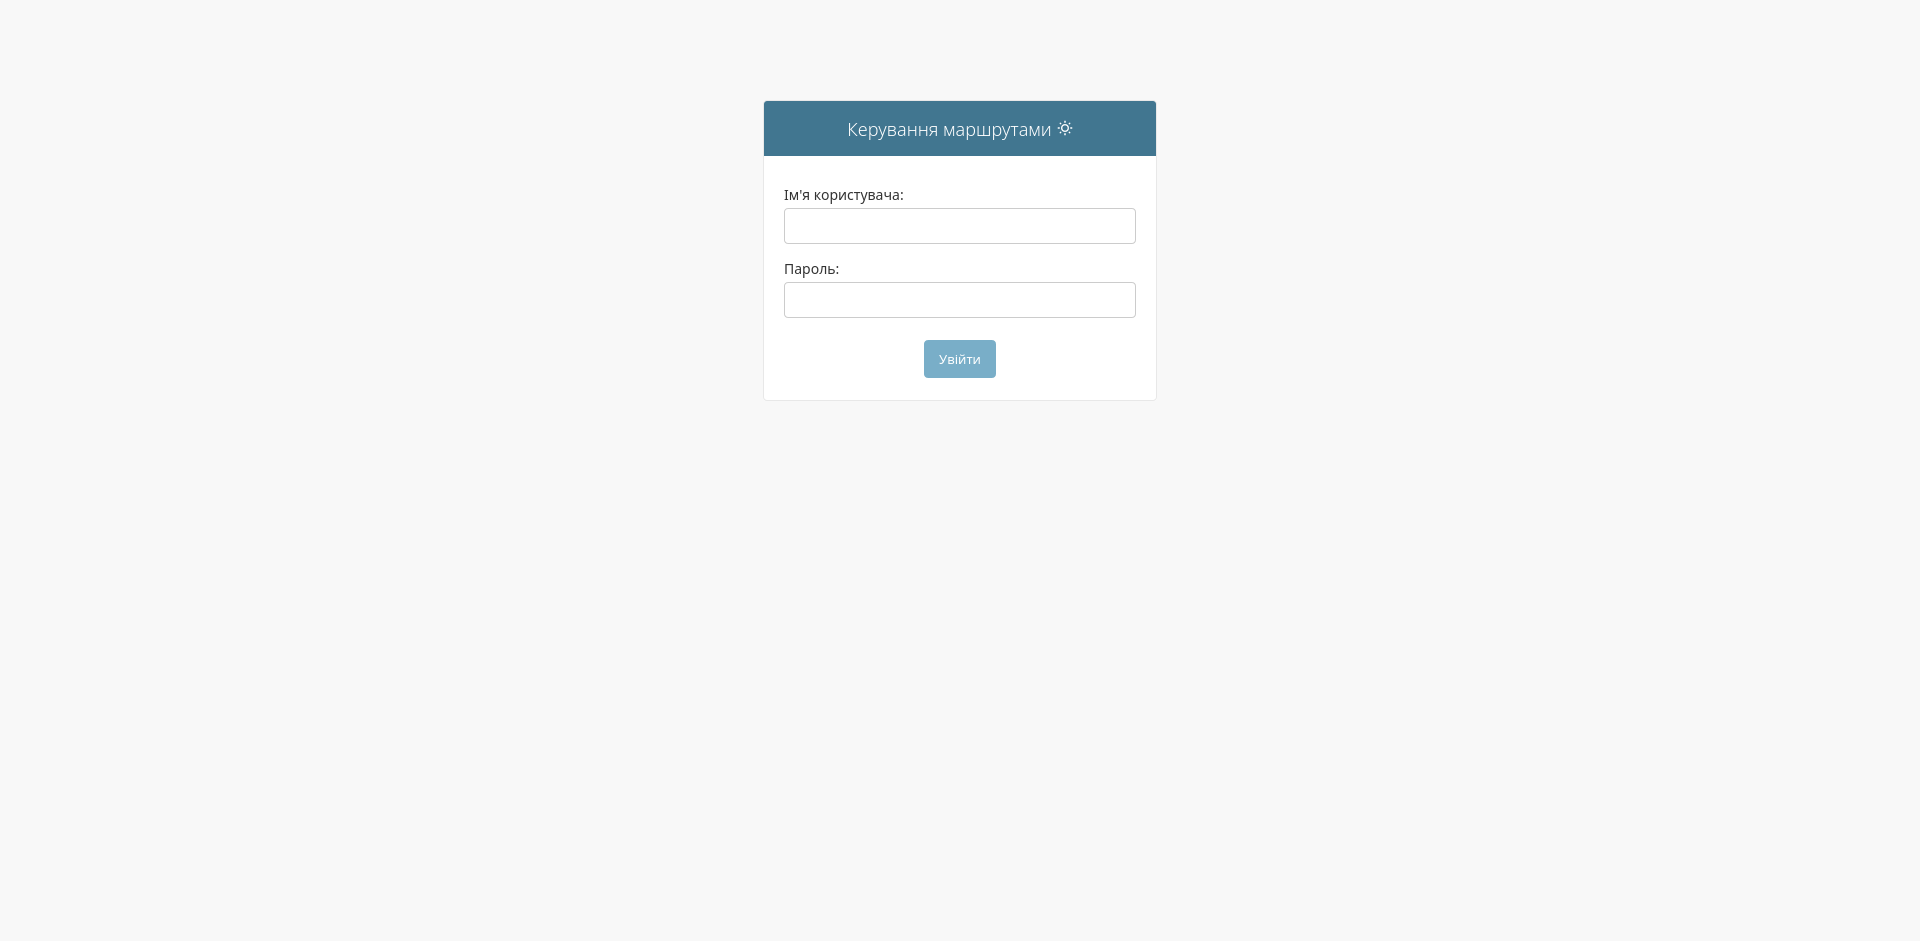
\includegraphics[scale=0.35]{content/chapters/4-results/assets/img/login_page.png}
	\caption{Сторінка входу}
	\label{fig:login_page}
\end{figure}

Можливості адміністратора буде розглянуто в наступному розділі

\subsection{Огляд можливостей управління транспортними даними}
\label{subsec:route-management-subsection}

Застосунок пропонує комплексний набір функцій управління транспортними даними, які дозволяють адміністраторам підтримувати та оновлювати базу даних транспортних маршрутів, розкладів та іншої пов'язаної з ними інформації. Ці функції дозволяють легко інтегрувати нові маршрути, вносити зміни до існуючих маршрутів та ефективно обробляти зміни в розкладі руху транспорту.

Однією з ключових особливостей функцій управління транспортними даними є можливість додавання нових транспортних маршрутів до системи. Адміністратори можуть вводити необхідні дані, такі як пункт відправлення, пункт призначення, проміжні зупинки та пов'язану з ними інформацію про розклад для кожного маршруту. Це дозволяє додатку надавати користувачам точні та вичерпні варіанти маршрутів під час пошуку.

Функції управління транспортними даними також включають можливість видалення застарілих або зайвих маршрутів із системи. Це гарантує, що додаток підтримує чисту та актуальну базу даних, підвищуючи ефективність процесу пошуку та покращуючи загальний користувацький досвід.

Для спрощення управління транспортними даними додаток надає інтуїтивно зрозумілі інтерфейси та інструменти, які полегшують навігацію та редагування інформації про маршрути. Адміністратори можуть використовувати ці інтерфейси для візуалізації маршрутів, перегляду розкладів і внесення необхідних змін у зручний для користувача спосіб. Система також може включати механізми перевірки даних для забезпечення точності та узгодженості введеної інформації, мінімізації помилок та покращення цілісності даних.

Використовуючи функції управління транспортними даними, адміністратори можуть ефективно підтримувати та оновлювати транспортні дані в додатку, забезпечуючи користувачам доступ до надійної та актуальної інформації про маршрути. Це дозволяє користувачам приймати обґрунтовані рішення, ефективно планувати свої поїздки та впевнено орієнтуватися в транспортній мережі.

Адміністратор може створювати нові маршрути для того щоб вони потім відображались при пошуку маршрутів

\begin{figure}[!h]
	\centering
	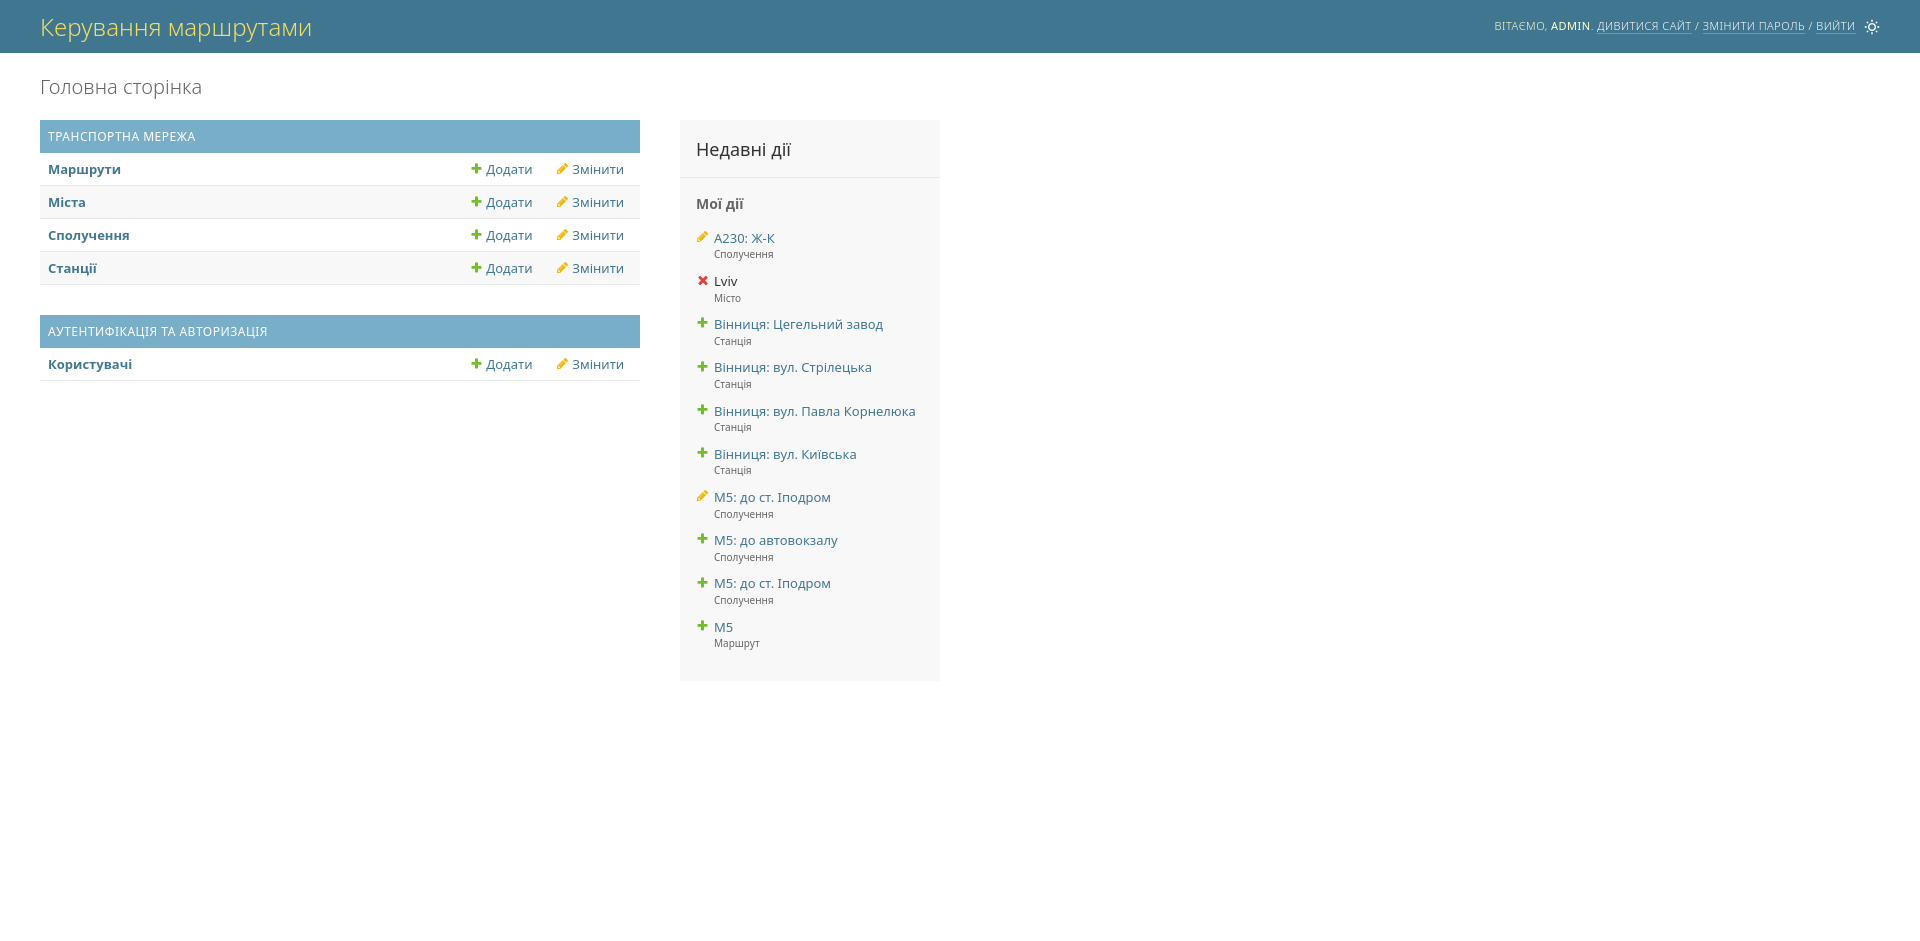
\includegraphics[scale=0.3]{content/chapters/4-results/assets/img/admin_main.png}
	\caption{Головна сторінка інрерфейсу адміна}
	\label{fig:admin_main_page}
\end{figure}

\begin{figure}[!h]
	\centering
	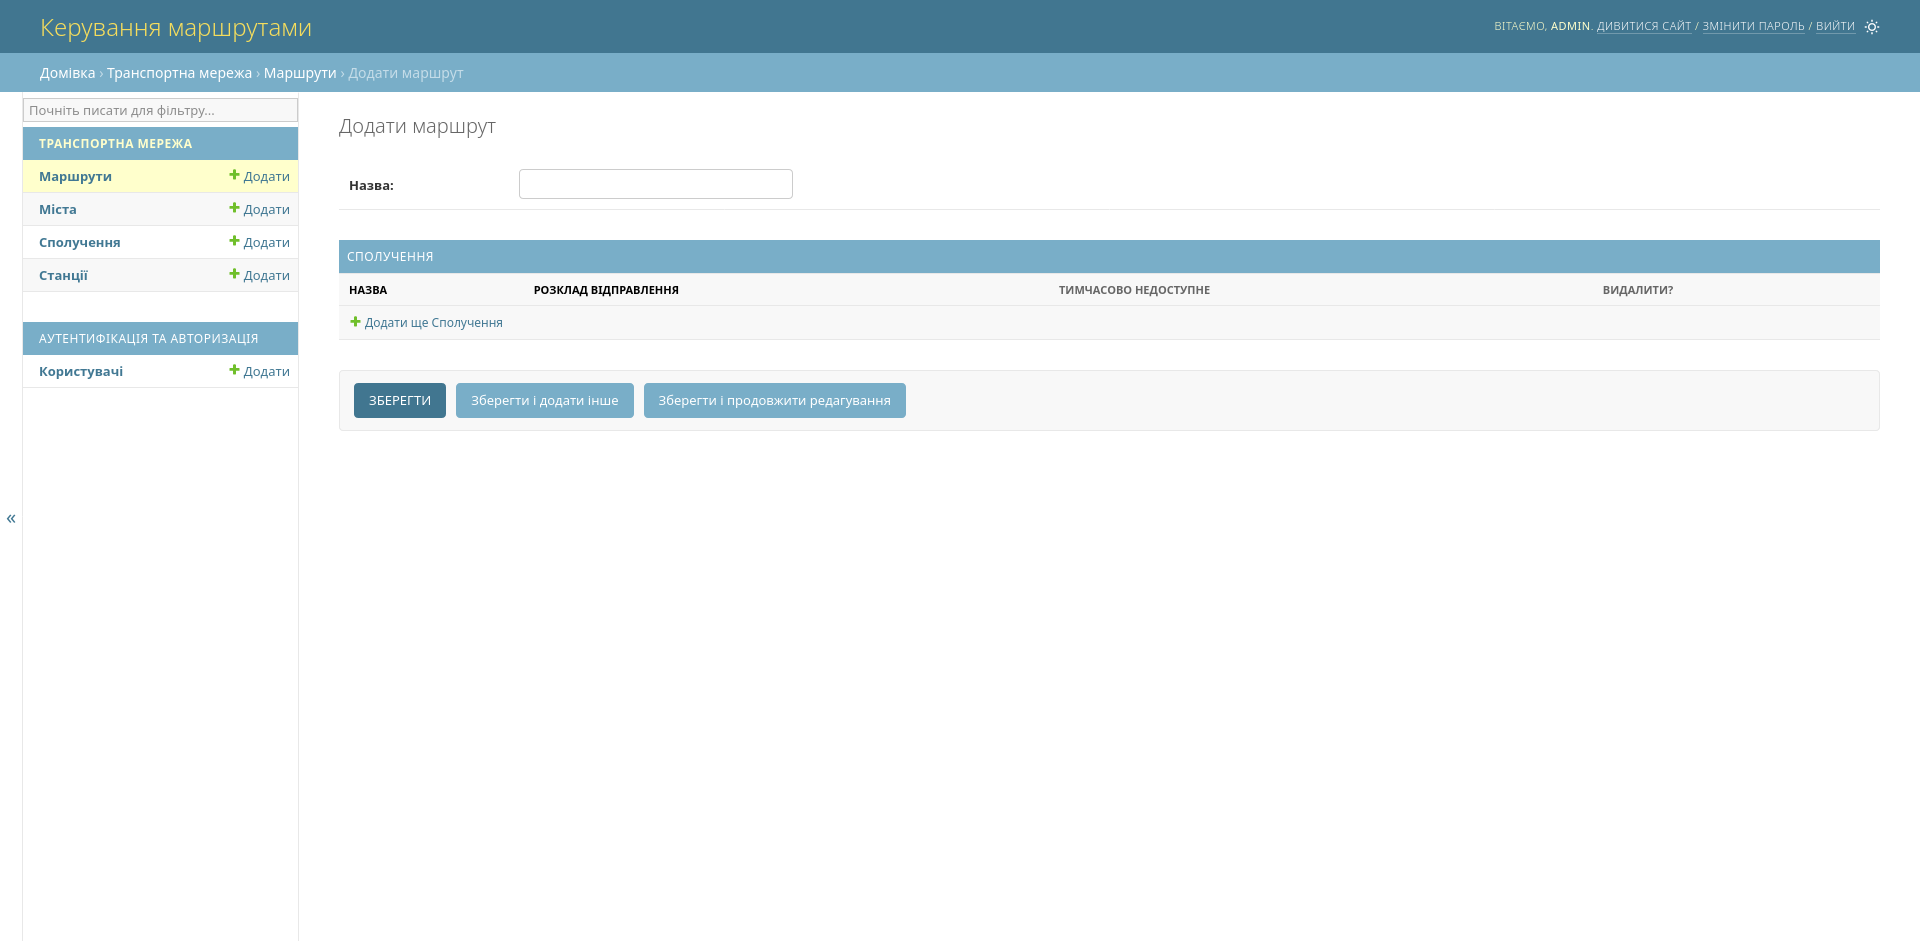
\includegraphics[scale=0.3]{content/chapters/4-results/assets/img/admin_create_r.png}
	\caption{Створення нового маршруту}
	\label{fig:roure_creation_page}
\end{figure}


\begin{figure}[!h]
	\centering
	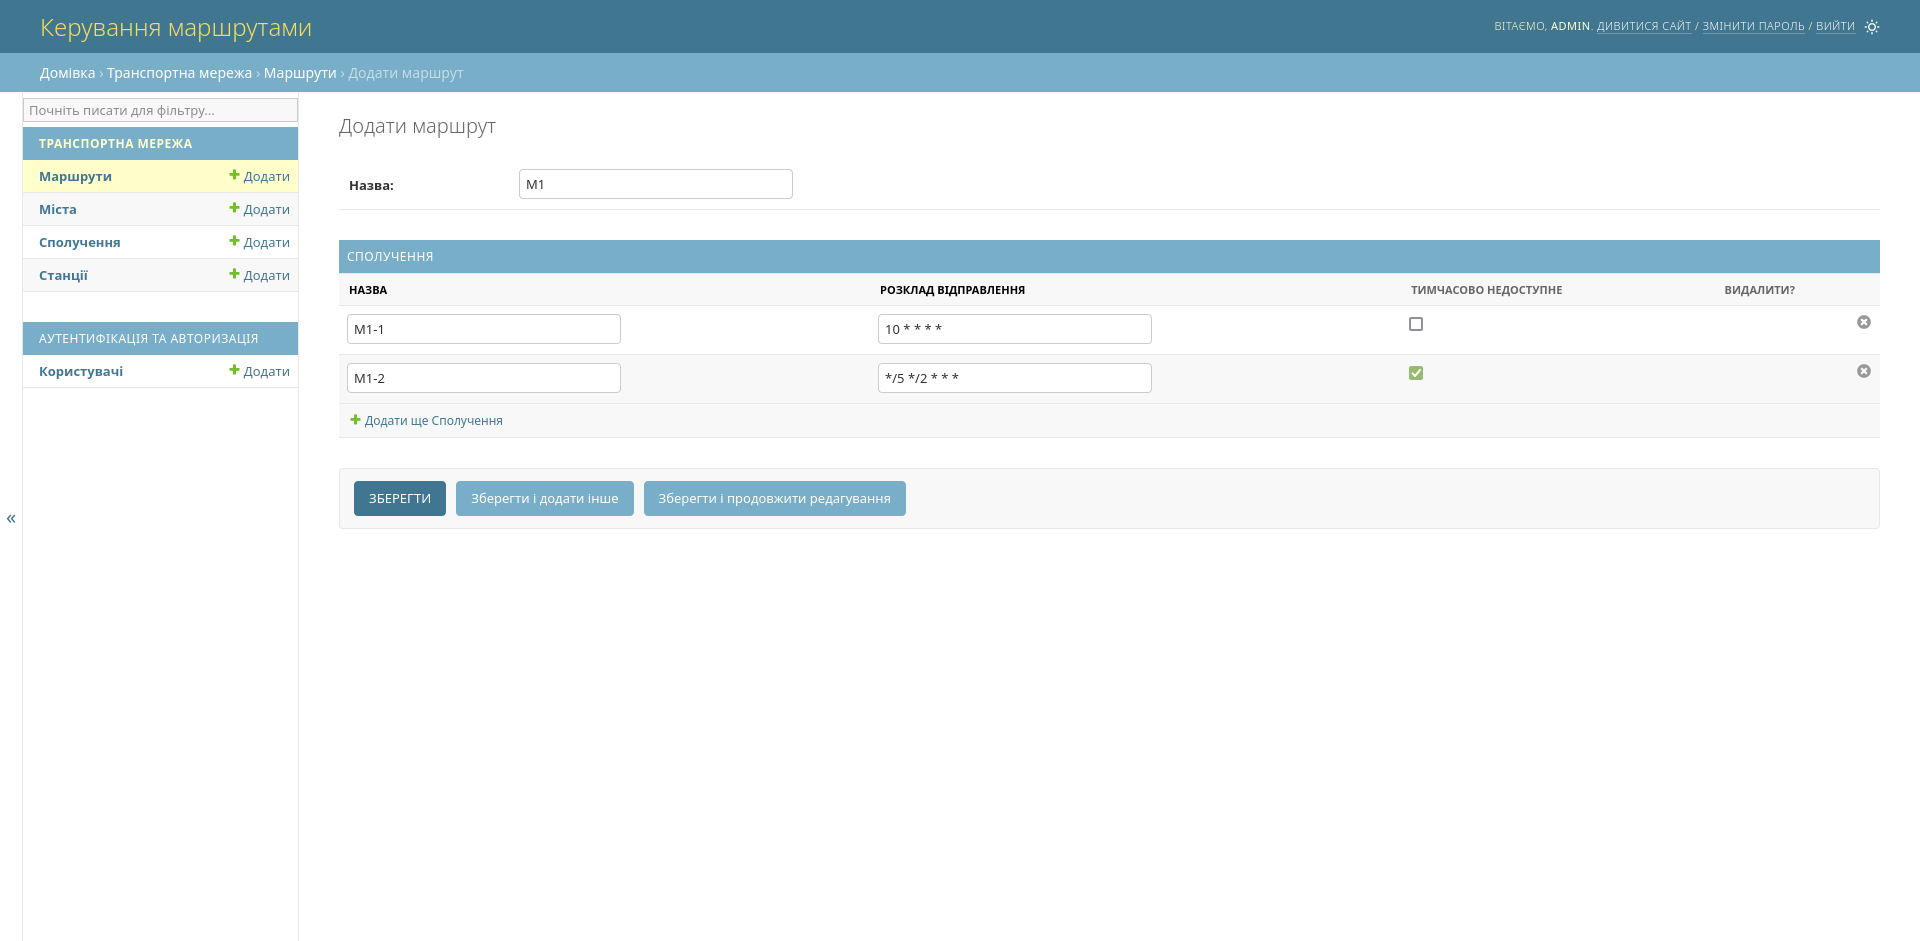
\includegraphics[scale=0.3]{content/chapters/4-results/assets/img/admin_create_R_filled.png}
	\caption{Заповнені поля для створення нового маршруту}
	\label{fig:route_creation_filled_page}
\end{figure}



Після створення маршрутів, їх можна переглядати в списку зі всіма маршрутами.

\begin{figure}[!h]
	\centering
	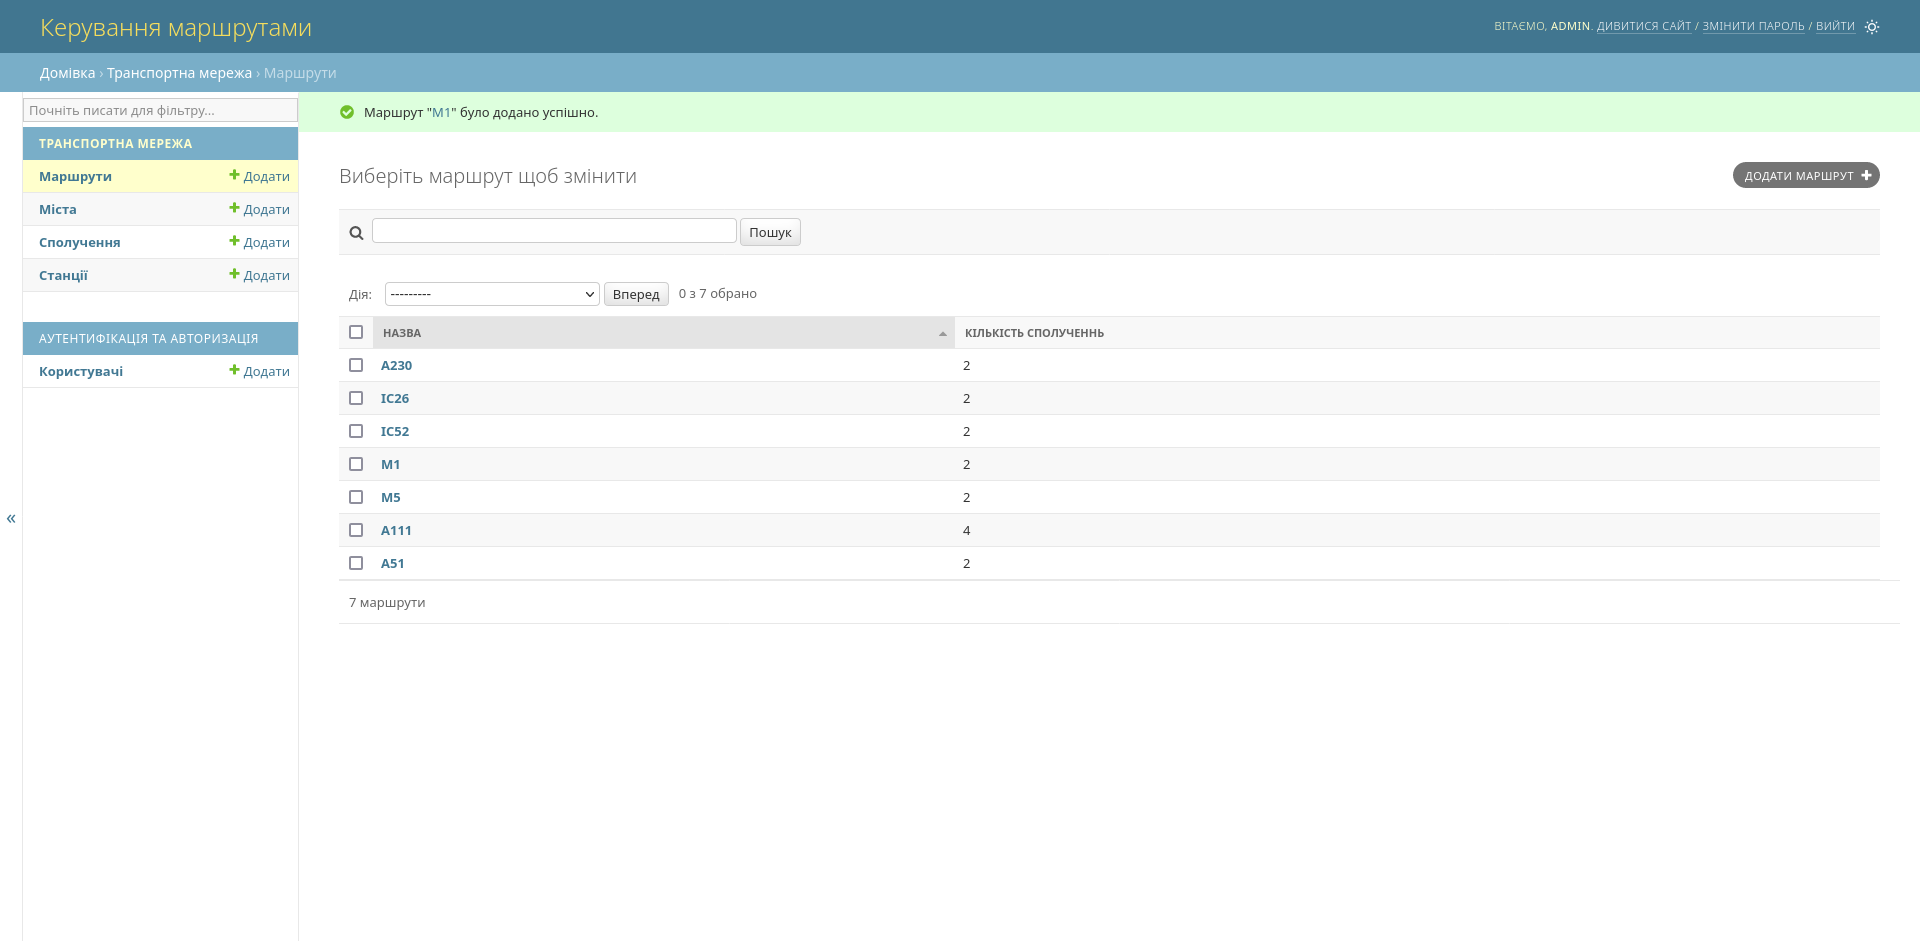
\includegraphics[scale=0.3]{content/chapters/4-results/assets/img/admin_view_r.png}
	\caption{Сторінка зі всіма маршрутами}
	\label{fig:route_display_page}
\end{figure}



Кожен маршрут можна відкрити на окремій сторінці для перегляду деталей  про нього. Якщо в маршруті є помилки, дані про маршрут можна редагувати, чи навіть видалити.

\begin{figure}[!h]
	\centering
	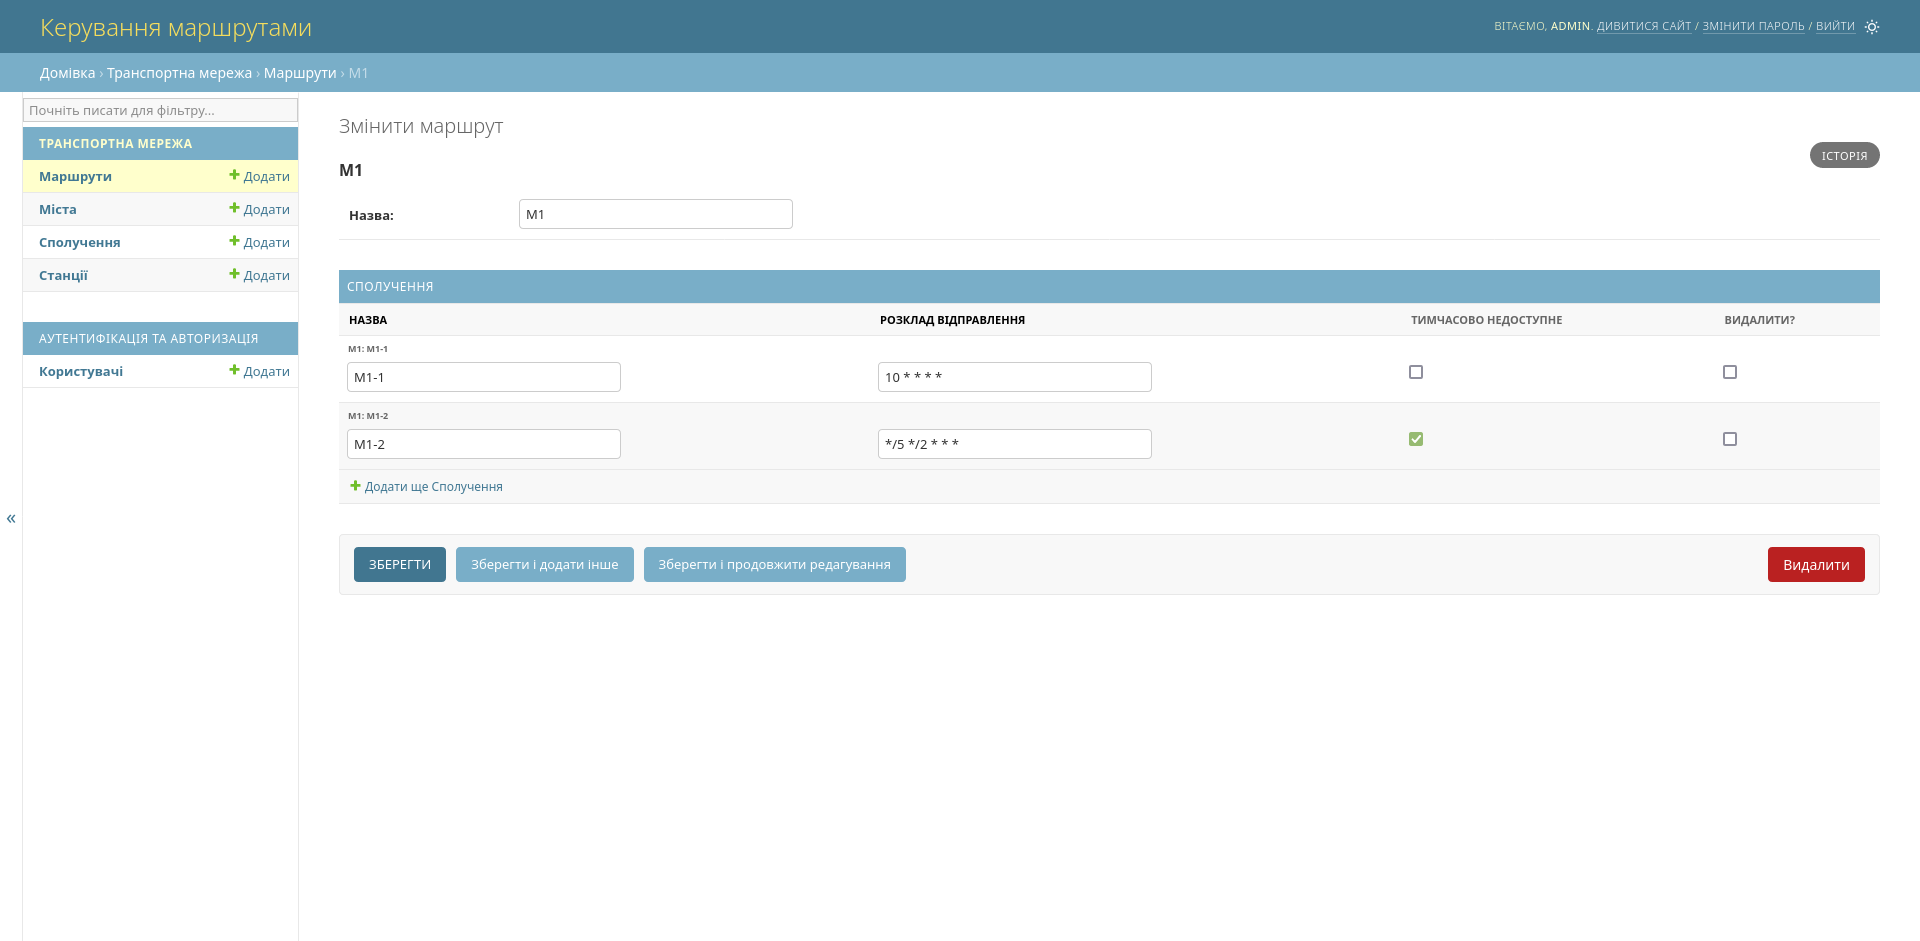
\includegraphics[scale=0.3]{content/chapters/4-results/assets/img/admin_r_details.png}
	\caption{Перегляд деталей про маршрут}
	\label{fig:route_edit_page}
\end{figure}
